\documentclass[11pt,usenames,dvipsnames,svgnames,x11names]{beamer} 

\usetheme{Warsaw}
\usepackage{amssymb,amsmath,amsthm,amsfonts}                    
\usecolortheme{whale} 
\setbeamertemplate{navigation symbols}{}
\usepackage[utf8]{inputenc} 
\usepackage{polski}
\usepackage{tikz}
\usepackage{subfigure}
\usepackage{setspace}
\usepackage{savesym}
\savesymbol{arc}
\usepackage{color}
\usepackage{xcolor}
\usepackage{pict2e}
\usepackage{epstopdf}
\usepackage{caption}
\usepackage{graphicx}
\usepackage{pict2e}
\usepackage{epstopdf}
\usepackage{geometry}
\usepackage{mathabx}

\date{8 kwietnia 2014}
\author{Marta Sommer}
\title{Przedział ufności dla mediany w~przypadku~populacji~dyskretnej}

\theoremstyle{plain}
\newtheorem{twierdzenie}{Twierdzenie} 
\newtheorem{twierdzeniecd}{Twierdzenie cd.} 
\theoremstyle{definition}
\newtheorem{definicja}{Definicja}
\newtheorem{przyklad}{Przykład}
\newtheorem{lemat}{Lemat}
\newtheorem{wniosek}{Wniosek}
\newtheorem{oznaczenia}{Oznaczenia}
\theoremstyle{remark}
\newtheorem{uwaga}{Uwaga}

\begin{document}


\begin{frame}   %tytułowa
\titlepage
\end{frame}

%%%%%%%%%%%%%%%%%%%%%%%%%%%%%%%%%%%%%%%%%%%%%%%%%%%%%%%%%%%%%%%%%%%%%%%%%%%%%%%%%%%%%%%%%%%%%%%%%%%%%%%%%%%%%%%%%%%%%

\begin{frame}
\frametitle{Test znaków}

\begin{center}
$X_1,X_2,\ldots,X_n$ -- obserwacje
\end{center}

Hipoteza:
$$
\left\{
\begin{array}{l}
H: M=M_0 \\
K: M\neq M_0 \\
\end{array}
\right.
$$
Statystyka testowa:
$$
T = \sum_{i=1}^n \mathbb{I}_{\lbrace X_i~>~M_0\rbrace } 
$$
Rozkład statystyki testowej:
$$
T\sim \operatorname{Bin}(n,\dfrac{1}{2})
$$
\end{frame}

\begin{frame}
\frametitle{Test znaków, cd.}
Hipotezę $H$ odrzucamy więc, gdy $T\geq k_{\frac{\alpha}{2}}$ lub $T\leq k_{\frac{\alpha}{2}}'$, gdzie $k_{\frac{\alpha}{2}}$~jest najmniejszą liczbą naturalną spełniającą nierówność:
$$
\sum_{i=k_{\frac{\alpha}{2}}}^n {n\choose i}\left(\dfrac{1}{2}\right)^n\leq \dfrac{\alpha}{2},
$$ 
zaś $k_{\frac{\alpha}{2}}'$ jest największą liczbą naturalną spełniającą nierówność:
$$
\sum^{k_{\frac{\alpha}{2}}'}_{i=0} {n\choose i}\left(\dfrac{1}{2}\right)^n\leq \dfrac{\alpha}{2}.
$$
Hipotezy $H$ nie odrzucamy natomiast w następującym przypadku:
$$
k_{\frac{\alpha}{2}}'<T<k_{\frac{\alpha}{2}}\hspace{1cm} \equiv \hspace{1cm} k_{\frac{\alpha}{2}}'+1 \leq T \leq k_{\frac{\alpha}{2}}-1.
$$
\end{frame}
 
\begin{frame}
\frametitle{Test znaków, cd.}
\begin{lemat}
Niech $r,s\in \{ 1,\ldots,n \}$, $r<s$ oraz niech $T$ będzie statystyką testu znaków. Wówczas prawdziwa jest teza:
$$
\mathbb{P}(X_{r:n}\leq M \leq X_{s:n}) = \mathbb{P}(r\leq T(X_1,\ldots,X_n)\leq s-1).
$$
\end{lemat}

$$
k_{\frac{\alpha}{2}}'+1 \leq T \leq k_{\frac{\alpha}{2}}-1
$$
Przyjmując $r:=k_{\frac{\alpha}{2}}'+1$ i $s:=k_{\frac{\alpha}{2}}$, otrzymujemy przedział ufności
$$
X_{(k_{\frac{\alpha}{2}}'+1):n}\leq M \leq X_{k_{\frac{\alpha}{2}}:n}
$$
na poziomie $1-\alpha$. 
\end{frame}

\begin{frame}
\frametitle{Problem}
\begin{uwaga}
Wszystkie te rozważania przeprowadzane są przy założeniach ciągłości rozkładu oraz zerowego prawdopodobieństwa wystąpienia mediany!
\end{uwaga}
\vspace{1.2cm}
Jak wygląda sytuacja dla rozkładu dyskretnego? Co dzieje się w przypadkach, gdy mediana występuje nawet kilkakrotnie? 
\end{frame}

\begin{frame}
\frametitle{Podstawowe oznaczenia}
Będziemy rozważać przedziały ufności oparte na statystyce porządkowej i mające następującą postać:
$$
[X_{d:n},X_{(n+1-d):n}]
$$
Dla populacji ciągłej powyższy przedział wyznaczony jest na~poziomie ufności równym
$$
1-\alpha = 1-2\cdot\mathbb{P}(B \leq d-1),
$$   
gdzie $B\sim\operatorname{Bin}(n,\dfrac{1}{2})$. 

\bigskip

Wynika to z dość prostego rachunku wykorzystującego to, że przy założeniu hipotezy zerowej $\mathbb{P}(B\geq t)=\mathbb{P}(B\leq n-t)$.
\end{frame}

\begin{frame}
\frametitle{Dowód}
$$\mathbb{P}(B\geq t)\stackrel{?}{=}\mathbb{P}(B\leq n-t)$$

\begin{eqnarray*}
\mathbb{P}(B\geq t)&=&\pause \left| \begin{array}{c}{\nonumber B\sim Bin(n,\dfrac{1}{2})}\end{array} \right| \pause \stackrel{H}{=} \sum_{i=t}^n {n \choose i} \left(\dfrac{1}{2}\right)^i\left(1-\dfrac{1}{2}\right)^{n-i}=\pause  \\&=&\sum_{i=t}^n {n \choose i} \left(\dfrac{1}{2}\right)^n\pause =\left(\dfrac{1}{2}\right)^n \sum_{i=t}^n {n \choose n-i}\pause=\\&=&\left(\dfrac{1}{2}\right)^n \sum_{i=0}^{n-t} {n \choose i}\pause =\sum_{i=0}^{n-t} {n \choose i} \left(\dfrac{1}{2}\right)^i\left(1-\dfrac{1}{2}\right)^{n-i}\pause =\\ &=&\mathbb{P}(B\leq n-t)
\end{eqnarray*}
\end{frame}

\begin{frame}
\frametitle{Dowód cd.}
$$
1-\alpha \stackrel{?}{=} 1-2\cdot\mathbb{P}(B \leq d-1)
$$
\begin{eqnarray*}
1&-&\alpha \pause = \mathbb{P}(M\in [X_{d:n},X_{(n+1-d):n}])\pause =\mathbb{P}(X_{d:n}\leq M \leq X_{(n+1-d):n})\pause =\\&=& \mathbb{P}(d\leq T \leq n+1-d-1)\pause =\mathbb{P}(d\leq T \leq n-d)\pause =\\&=&\mathbb{P}(T \leq n-d)-\mathbb{P}(T < d)\pause =\mathbb{P}(T \leq n-d)-\mathbb{P}(T \leq d-1)\pause =\\&=&\mathbb{P}(T \geq d)-\mathbb{P}(T \leq d-1)\pause =1-\mathbb{P}(T<d)-\mathbb{P}(T\leq d-1)\pause =\\&=& 1-\mathbb{P}(T\leq d-1)-\mathbb{P}(T\leq d-1)\pause =1-2\cdot \mathbb{P}(T\leq d-1)
\end{eqnarray*}
\end{frame}

\begin{frame}
\frametitle{Problem}
\begin{uwaga}
Prawdziwym problemem jest określenie \underline{poziomu ufności} dla znalezionego już przedziału ufności.
\end{uwaga}
Ze względu na to, że dane są dyskretne, istnieje skończenie wiele (ewentualnie przeliczalnie wiele) możliwych przedziałów ufności, a~tym samym -- skończenie wiele poziomów ufności możliwych do osiągnięcia. 
\end{frame} 

\begin{frame}
\frametitle{Metoda 1}
Poziom ufności wyznaczamy wprost ze wzoru
$$
1-\alpha = 1-2\cdot\mathbb{P}(B \leq d-1),
$$
ignorując to, że dane są dyskretne. 
\end{frame}

\begin{frame}
\frametitle{Metoda 2}
Rozważamy poziomy ufności wyznaczone tym samym wzorem, co~w metodzie 1, dla przedziału ufności $[X_{d:n},X_{(n+1-d):n}]$:
$$
1-\alpha = 1-2\cdot\mathbb{P}(B \leq d-1)
$$
oraz poziomy ufności wyznaczone dla nieznacznie niesymetrycznego przedziału ufności $[X_{(d+1):n},X_{(n+1-d):n}]$:
$$
1-\alpha = 1-\mathbb{P}(B \leq d-1)-\mathbb{P}(B \leq d).
$$
Wyznaczamy wszystkie możliwe przedziały i wybieramy ten, który ma najmniejszy poziom ufności większy lub równy $0,95$. 
\end{frame}

\begin{frame}
\frametitle{Metoda 3}
Rozważamy symetryczny przedział ufności $$[X_{d:n},X_{(n+1-d):n}].$$ Stosując tę metodę, weźmiemy pod uwagę ewentualne obserwacje związane.

Niech $r$ będzie najmniejszym indeksem, dla którego $$X_{r:n}=X_{d:n}$$ oraz niech $s$ będzie największym indeksem, dla którego $$X_{s:n}=X_{(n+1-d):n}$$ 

Poziom ufności wyraża się wtedy wzorem:
$$
1-\alpha = 1-\mathbb{P}(B \leq r-1)-\mathbb{P}(B \leq n-s).
$$
\end{frame}

\begin{frame}
\frametitle{Wstęp do metod 4--7}
Rozważamy przedział ufności $[X_{d:n},X_{(n+1-d):n}].$

Metody te stosuje się, opierając się na odwróceniu dwustronnego testu znaków z obserwacjami związanymi. 

Poziom ufności wyraża się następująco:
$$
1-\alpha = 1- \max{\lbrace p.value(X_{d:n}-), p.value(X_{(n+1-d):n}+) \rbrace},
$$
gdzie $p.value(c)$ to p-value dwustronnego testu o hipotezie:
$$
\left\{
\begin{array}{l}
H: M=c \\
K: M\neq c \\
\end{array}
\right.
$$
$X_{d:n}-$ oznacza pierwszą możliwą obserwację poniżej $X_{d:n}$, zaś $X_{(n+1-d):n}+$ oznacza pierwszą możliwą obserwację powyżej $X_{(n+1-d):n}$.
\end{frame}

\begin{frame}
\frametitle{Metoda 4}
Korzystając z p-value wyznaczonego dla dwustronnego testu znaków przy założeniu ciągłości rozkładu, przyjmiemy:
$$
p.value(c) = 2\cdot\mathbb{P}(B\leq \min{\lbrace n_+^c,n_-^c\rbrace}),
$$
gdzie $n_+^c$ to liczba obserwacji większych niż $c$, zaś $n_-^c$ to liczba obserwacji mniejszych niż $c$.
\end{frame}

\begin{frame}
\frametitle{Wstęp do metod 5--7}
Rozważmy teraz sytuację podobną do tej z metody 4, biorąc jednak pod uwagę, że mamy do czynienia z rozkładem dyskretnym. W szczególności możemy przyjąć, że $X_{d:n}- = X_{d:n}-1$, a $X_{(n+1-d):n}+ = X_{(n+1-d):n}+1$. Wtedy:
$$
1-\alpha = 1- \max{\lbrace p.value(X_{d:n}-1), p.value(X_{(n+1-d):n}+1) \rbrace}.
$$
Może się jednak zdarzyć, że obserwacja $X_{d:n}-1$ nie wystąpi wcale lub wystąpi kilkakrotnie. Należy zatem policzyć p-value, biorąc pod~uwagę obserwacje związane.  
\end{frame}

\begin{frame}
\frametitle{Wstęp do metod 5--7}
Wprowadźmy następujące oznaczenia:

$n_+^c$ -- liczba obserwacji większych niż $c$,

$n_-^c$ -- liczba obserwacji mniejszych niż $c$,

$n_0^c$ -- liczba obserwacji równych $c$.

\bigskip

Rozważmy dwustronny test znaków, który odrzuca hipotezę dla dużych wartości
$$
n_*^c = \max{\lbrace n_+^c,n_-^c \rbrace}.
$$
P-value takiego testu będzie wyglądała następująco:
$$
p.value(c) = \mathbb{P}(N_*\geq n_*^c | \stackrel{\sim}{p}_+,\stackrel{\sim}{p}_-,\stackrel{\sim}{p}_0),
$$
gdzie $N_* = \max{\lbrace N_+,N_- \rbrace}$, a $(N_+,N_0,N_-)$ ma rozkład wielomianowy z parametrami $n$ i $(\stackrel{\sim}{p}_+,\stackrel{\sim}{p}_0,\stackrel{\sim}{p}_-)$, które spełniają warunki:
$ 0 \leq  \stackrel{\sim}{p}_+ \leq \frac{1}{2}$ oraz $ 0 \leq  \stackrel{\sim}{p}_- \leq \frac{1}{2}$.
\end{frame}

\begin{frame}
\frametitle{Wstęp do metod 5--7}
Ustaliwszy parametry $(\stackrel{\sim}{p}_+,\stackrel{\sim}{p}_0,\stackrel{\sim}{p}_-)$, wyznaczymy p-value, a~tym~samym poziom ufności.

\bigskip

Metody 5--7 pozwolą na różne sposoby przybliżać wartości $(\stackrel{\sim}{p}_+,\stackrel{\sim}{p}_0,\stackrel{\sim}{p}_-)$. 
\end{frame}

\begin{frame}
\frametitle{Metoda 5}
Dla $n_*^c \leq \dfrac{n}{2}$:
$$
\stackrel{\sim}{p}_{+mle} = \dfrac{n_+^c}{n},\hspace{1cm}\stackrel{\sim}{p}_{0mle} = \dfrac{n_0^c}{n},\hspace{1cm}\stackrel{\sim}{p}_{-mle} = \dfrac{n_-^c}{n}
$$
Dla $n_+^c > \dfrac{n}{2}$:
$$
\stackrel{\sim}{p}_{+mle} = \dfrac{1}{2},\hspace{1cm}\stackrel{\sim}{p}_{0mle} = \dfrac{n_0^c}{2(n-n^c_+)},\hspace{1cm}\stackrel{\sim}{p}_{-mle} = \dfrac{n_-^c}{2(n-n^c_+)}
$$
Dla $n_+^c = n$:
$$
\stackrel{\sim}{p}_{+mle} =\stackrel{\sim}{p}_{-mle} = \dfrac{1}{2},\hspace{1cm} \stackrel{\sim}{p}_{0mle}=0 
$$
Analogicznie dla $n_-^c> \dfrac{1}{2}$.
\end{frame}

\begin{frame}
\frametitle{Metoda 6}
Szukamy $(\stackrel{\sim}{p}_+,\stackrel{\sim}{p}_0,\stackrel{\sim}{p}_-)$, minimalizując wyrażenie:
$$
\left(\dfrac{n_+^c}{n}-p_+\right)^2 + \left(\dfrac{n_0^c}{n}-p_0\right)^2 + \left(\dfrac{n_-^c}{n}-p_-\right)^2
$$
przy warunkach $ 0 \leq  \stackrel{\sim}{p}_+ \leq \frac{1}{2}$ oraz $ 0 \leq  \stackrel{\sim}{p}_- \leq \frac{1}{2}$.

\bigskip

Rozwiązania tego problemu wyglądają następująco:
$$
\stackrel{\sim}{p}_{+cql} = \dfrac{n_+^c}{n},\hspace{1cm}\stackrel{\sim}{p}_{0cql} = \dfrac{n_0^c}{n},\hspace{1cm}\stackrel{\sim}{p}_{-cql} = \dfrac{n_-^c}{n},
$$
dla $n_*^c \leq \dfrac{n}{2}$.
$$
\stackrel{\sim}{p}_{+cql} = \dfrac{1}{2},\hspace{0.6cm}\stackrel{\sim}{p}_{0cql} = \dfrac{n_0^c}{n} + \dfrac{1}{2}\left( \dfrac{n_+^c}{n} - \dfrac{1}{2} \right),\hspace{0.6cm}\stackrel{\sim}{p}_{-cql} = \dfrac{n_-^c}{n} + \dfrac{1}{2}\left( \dfrac{n_+^c}{n} - \dfrac{1}{2} \right),
$$
dla $n_+^c > \dfrac{n}{2}$. Analogicznie dla $n_-^c> \dfrac{1}{2}$.
\end{frame}

\begin{frame}
\frametitle{Metoda 7}
Jest nieznaczną modyfikacją metody 6. 

\bigskip

Dla $n_0^c > 0$ zachodzi równość $(\stackrel{\sim}{p}_+,\stackrel{\sim}{p}_0,\stackrel{\sim}{p}_-) = (\stackrel{\sim}{p}_{+cql},\stackrel{\sim}{p}_{0cql},\stackrel{\sim}{p}_{-cql})$.

\bigskip

Zmiana następuje dla $n_0^c = 0$. Ma wtedy miejsce równość$$(\stackrel{\sim}{p}_+,\stackrel{\sim}{p}_0,\stackrel{\sim}{p}_-) = \left( \dfrac{1}{2},0,\dfrac{1}{2} \right).$$

\end{frame}

\begin{frame}
\frametitle{Porównanie metod}
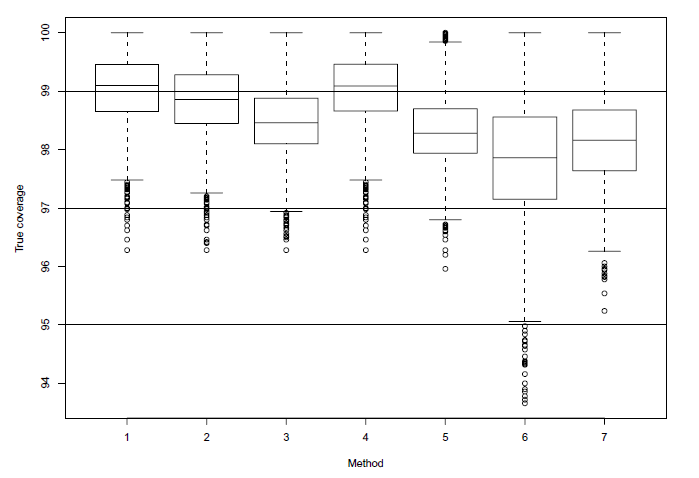
\includegraphics[width=\textwidth]{1.png}
\end{frame}

\begin{frame}
\frametitle{Porównanie metod, cd.}
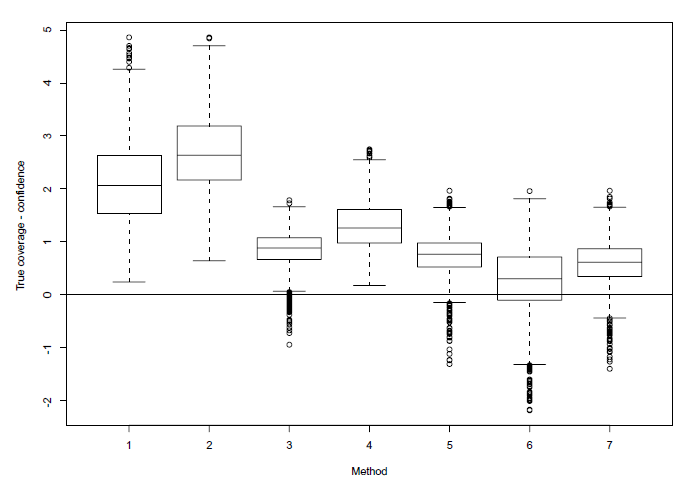
\includegraphics[width=\textwidth]{2.png}
\end{frame}

\begin{frame}
\frametitle{Porównanie metod}
\centering
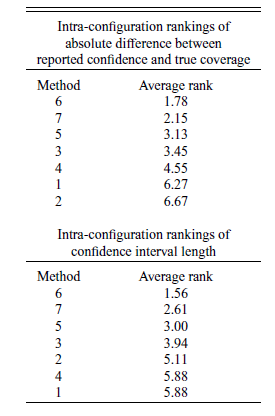
\includegraphics[width=0.5\textwidth]{4.png}
\end{frame}

\begin{frame}
\frametitle{Porównanie metod}
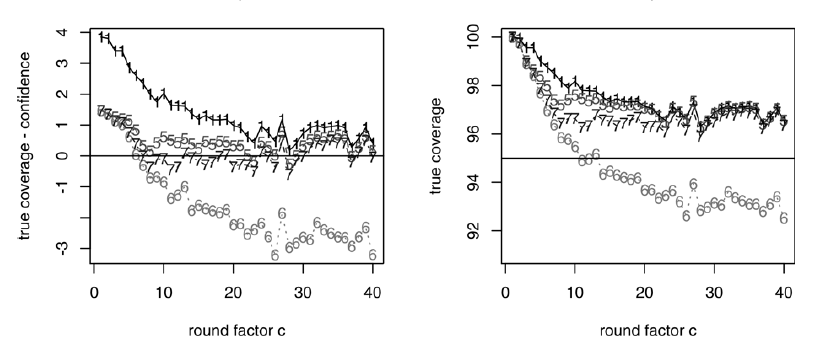
\includegraphics[width=\textwidth]{3.png}
\end{frame}

\begin{frame}
\frametitle{Porównanie metod}
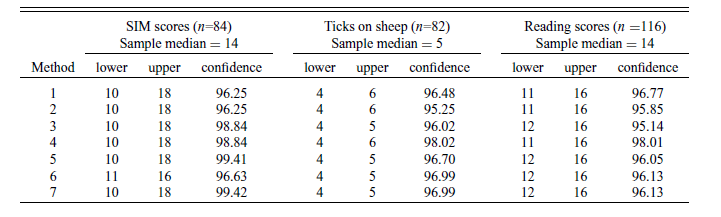
\includegraphics[width=\textwidth]{5.png}
\end{frame}

\begin{frame}
\frametitle{Bibliografia}
\begin{thebibliography}{9}
\bibitem{budyn1} Larocque, Denis, Randles, Ronald H. Confidence Intervals for a Discrete Population Median, \emph{The American Statistician} 2008, nr 62, s. 32--39.
\bibitem{budyn2} Emerson, J.D., Simon, G.A. Another Look at the Sign Test when Ties are Present: the Problem of Confidence Intervals, \emph{The American Statistician} 1979, nr 33, s. 140--142.
\bibitem{budyn3} Fong, D.Y.T., Kwan, C.W., Lam, K.F., Lam, K.S.L. Use of the Sign Test for the Median in the Presence of Ties, \emph{The American Statistician} 2003, nr 58, s. 237--240.
\end{thebibliography}
\end{frame}








\end{document}
